\begin{lstlisting}
实现:就是量子门集合

添加量子门的方法:
1. +=
2. circuit.x
3. list

展示线路的方法:svg

介绍常用接口:
1. n_qubits(包含多少比特)
2. params_name(有哪些变量)
3. has_measure_gate(是否含有测量)
4. matrix()(获取线路矩阵)
5. get_qs()(获取量子态)
6. summary()

高阶操作:
1. 线路压缩
2. 更改比特顺序
3. 更改变量名
\end{lstlisting}

The quantum circuit can accomplish some useful tasks, it can change the states of the qubits. The quantum circuit is to be read from left-to-right. Each line in the circuit represents a \textit{wire} in the quantum circuit. This wire does not necessarily correspond to a physical wire; it may correspond instead to the passage of time, or perhaps to a physical particle. 

There are a few features allowed in classical circuits that are not usually present in quantum circuits. First of all, we do not allow 'loops', that is, feedback from one part of the quantum circuit to another. second, classical circuits allow wires to be 'joined' together. Third, the inverse operation is also not allowed in quantum circuits.

The quantum circuit has some important operations. First, it allows us to use control qubit to operator on the target qubit, if the control qubit is set 1 then the gate will be applied to the targer qubits. Another important operation is measurement, which we represent by a 'meter' symbol.  
 
\subsection{Quantum gate set}
Quantum gates (quantum logic gates) are the basic logical units of quantum circuit. Basic quantum gates commonly used are X gate, Y gate, Z gate, Hadamard gate (H gate), CNOT gate, and revolving gate RX gate, RY gate, and RZ gate. \\

\textbf{1. X, Y, Z gate}

X, Y, Z gate are Pauli matrices, they are single qubit gates and operator on single qubit, can rotate $\pi$ angles around the X, Y and Z axis of the Bloch sphere.   \\

\textbf{2. Hadamard(H) gate}

matrix representation: $H = \frac{1}{\sqrt{2}} \left( \begin{array}{cc}
     1 & 1 \\
     1 & -1 
\end{array} \right)$  

H gate is also single qubit gate, but it can change the ground state to a superposition state. \\

\textbf{3. CNOT gate}

matrix representation: $CNOT = \left( \begin{array}{cccc}
     1 & 0 & 0 & 0 \\
     0 & 1 & 0 & 0 \\
     0 & 0 & 0 & 1 \\
     0 & 0 & 1 & 0
\end{array} \right)$  

CNOT gate is a two-qubit gate, it can operator controll qubit and target qubit. \\

\textbf{4. RX, RY, RZ gate}

RX, RY, RZ can rotate the quantum state $\theta$ angles around the X, Y and Z axes on a Bloch sphere. RX, RY can bring about a change in probability amplitude, and RZ only a change in phase.
\subsection{Add quantum gate}
Mindquantum has libraries associated with quantum gates, which can be used to operate on quantum gates. 
\begin{lstlisting}
from mindquantum.core.gates import X, Y, Z, H, RX, RY, RZ
from mindquantum.core.circuit import Circuit
encoder = Circuit()
\end{lstlisting}

There are several basic operations for adding a quantum gate.
\begin{itemize}
    \item +=: use '+=' to add a quantum gate to the circuit.
    \item Circuit.x: add an X gate to the circuit.
    \item list: Circuit allows multiple bits to be operated on simultaneously, passing data of the same type as a list.  
\end{itemize}
\begin{lstlisting}
encoder += H.on(0) 
encoder += Y.on(1, 0)
encoder.x(1, 0)
encoder.z(2, [0, 1])        
\end{lstlisting}
\subsection{SVG}
SVG(Scalable Vector Graphics) is based on the XML markup language and is used to describe vector graphics in two dimensions. Mindquantum provides a function to save the picture in SVG format.
\begin{lstlisting}
encoder.svg().to_file(filename='circuit.svg')
\end{lstlisting}
    \begin{figure}[h]
       \begin{center}
            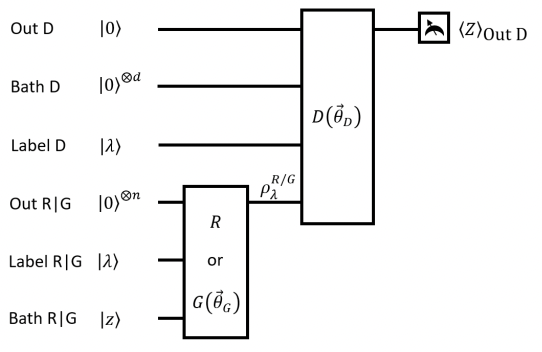
\includegraphics[width=0.5\linewidth]{images/circuit.png}
        \end{center}
        \caption{quantum circuit}
    \end{figure}
\subsection{API}
Mindquantum provides several common API for quantum circuit.
\begin{itemize}
    \item n\_qubits: get the number of qubit of quantum circuit.
    \item params\_name: get the params of circuit.
    \item has\_measure\_gate: get whether to be measured.
    \item matrix(): get the circuit matrix.
    \item get\_qs(): get the final quantum state.
    \item summary(): get information about the current circuit, including the number of blocks、 gates、 gates without parameters、 gates with parameters and parameters.
\end{itemize}
\begin{lstlisting}
encoder.n_qubits
encoder.params_name
encoder.has_measure_gate
encoder.matrix() 
encoder.get_qs()
encoder.summary()
\end{lstlisting}
Output:
\begin{lstlisting}
3
[]
False
[[ 0.70710678+0.j          0.        +0.70710678j  0.        +0.j
   0.        +0.j          0.        +0.j          0.        +0.j
   0.        +0.j         -0.        +0.j        ]
 ......
 [ 0.        +0.j          0.        +0.j          0.        +0.j
   0.        +0.j          0.        +0.j          0.        +0.j
   0.70710678+0.j         -0.        -0.70710678j]]
   
[ 0.70710678+0.j          0.        +0.70710678j  0.        +0.j
  0.        +0.j          0.        +0.j          0.        +0.j
  0.        +0.j         -0.        +0.j        ]
  
=======Circuit Summary=======
|Total number of gates  : 4.|
|Parameter gates        : 0.|
|with 0 parameters are  :   |
|                        .  |
|Number qubit of circuit: 3 |
=============================  
\end{lstlisting}
\subsection{Advanced operator}
Mindquantum also provides several Advanced API for quantum circuit.
\begin{itemize}
    \item compress(): delete all unused qubits and map the qubits to range(n\_qubits).
    \item SwapParts(a: Iterable, b: Iterable, maps\_ctrl=None): swapping a and b of a quantum circuit and can add control bits maps\_ctrl.
    \item change\_param\_name(circuit\_fn, name\_map): change parameter names in parametric quantum circuits or parametric quantum operators.
\end{itemize}
\begin{lstlisting}
encoder.compress()

from mindquantum.core.circuit import SwapParts
SwapParts([0, [1, 2], 0) 

from mindquantum.core.circuit import change_param_name
encoder.rx('a')
encoder1 = change_param_name(encoder, {'a': 'b'})  
\end{lstlisting}